% Chapter Template

% \chapter{Proposed Methodology II} % Main chapter title

% \label{chp:proposed2} % Change X to a consecutive number; for referencing this chapter elsewhere, use~\ref{ChapterX}


CNN, like many computer vision models, is a scale-variant~\cite{van2017learning} model such that it cannot recognize objects at various scales unless it explicitly trained to recognize such objects. Data augmentation can accomplish some degree of invariance as it allows the network to be trained with distorted samples, but it not the case for pneumonia scales. This chapter presents a CNN architecture that learns multiscale features using scale pyramid of the  CNN's internal feature maps. Scale pyramid is constructed using atrous convolution of various dilation rates. The correct scale from scale pyramid that allows minimization of the objective function loss is selected using the spatial attention mechanism. 
\section{Methodology II} 

\begin{center}
    \begin{figure*}[htbp]
    \centerline{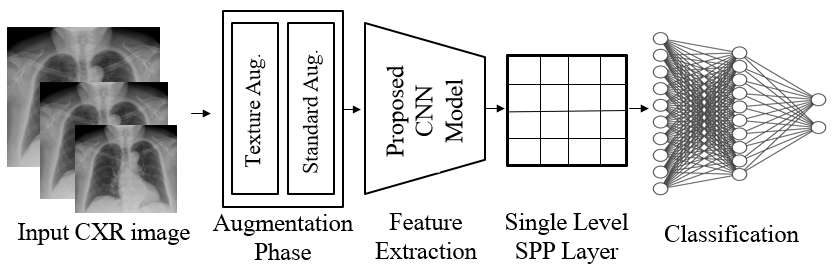
\includegraphics[height=40mm,width=15cm]{Figures/ProposedPipe.png}}
    \caption{Proposed method for COVID-19 classification from CXR images.}\label{ProposedPipe}\end{figure*}\end{center}
    
The proposed system presented in this chapter proposes a novel CNN micro-architecture model for learning scale-invariant features from row input CXR images and then classifies these features into normal or COVID-19 cases. Fig.~\ref{ProposedPipe} illustrates trainable end-to-end pipeline of the proposed system. The proposed system depends on a novel Spatially weighted Atrous Spatial Pyramid Pooling (SWASPP) to extract multi-scale features of input CXR images. A novel attention module is then used to fuse the extracted these multi-scale features and select relevant features' scale that the next layer should consider.
\subsection{Data augmentation}

\begin{center}
    \begin{figure}[htbp]
    \centerline{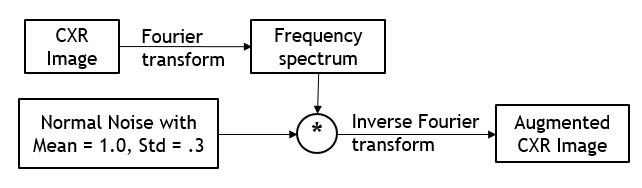
\includegraphics[height=30mm,width=9cm]{Figures/TexAug.PNG}}
    \caption{Texture Augmentation module}
    \label{texaug}
    \end{figure}
    \end{center}
The first phase of the proposed CXR classification system is data augmentation phase. Data augmentation is used to reduce the overfitting by artificially enlarge the training dataset~\cite{krizhevsky2012imagenet} using label preserving transformation. Data augmentation phase introduces a degree invariance to a distortion transformation such as the flipping and rotation. The input CXR images are augmented using texture augmentation.  Texture augmentation is performed by introducing a multiplicative normally distributed noises to the frequency spectrum of the input image. CXR image is transformed to the frequency spectrum using the fourier transform.  Noise is modeled using $\mathcal{N}(\mu = 1,\,\sigma = 0.3)$. Fig.~\ref{texaug} illustrates texture augmentation process for frequency distortion of the CXR image. Fig.~\ref{resltaug} shows the original CXR image and the corresponding frequency distorted CXR image. A standard augmentation techniques such as random rotation, horizontal flipping, and vertical flipping are included in the augmentation process. 

\begin{center}
    \begin{figure}[htbp]
    \centerline{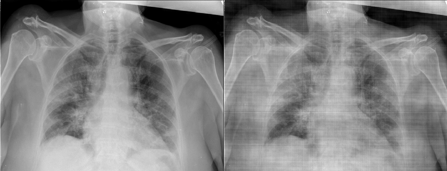
\includegraphics[height=40mm,width=9cm]{Figures/freqJitt.png}}
    \caption{Texture Augmentation}{The resulting CXR image from Texture augmentation \textbf{left}: is the original image. \textbf{Right} is the augmented  CXR Image}
    \label{resltaug}
    \end{figure}
    \end{center} 
    

\begin{center}
\begin{figure}[htbp]
\centerline{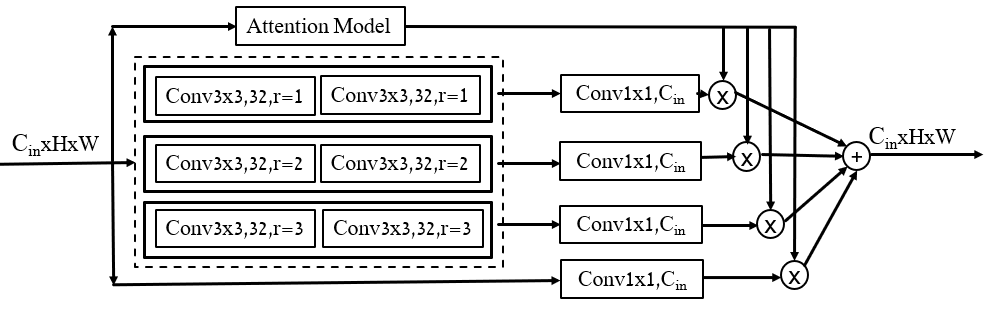
\includegraphics[height=50mm,width=9cm]{Figures/SWASPP.PNG}}
\caption{Spatially weighted atrous spatial Pyramid Pooling (SWASPP) interal layers within dashed square are parameter shared.}
\label{swaspp}
\end{figure}
\end{center}

\subsection{Spatially Weighted Atrous Spatial Pyramid Pooling}

Atrous convolution is a powerful technique for adjusting the resolution of convolutional kernels. This allows to effectively enlarge the field-of-view of the kernel without increasing neither the number of kernel parameters nor the computational complexity of the convolution operation. Atrous convolution is equivalent to performing downsampling and then performing convolution with original kernel without dilation. As a result different dilation rates of the kernel corresponding to different downsampling degrees. A novel spatially weighted atrous spatial pyramid pooling (SWASPP) micro-architecture is presented that exploit the scale space of the CNN's feature maps. Fig.~\ref{swaspp} shows the architecture of the SWASPP. In Fig.~\ref{swaspp}, internal pipelines, bounded by dashed-line square, are parameter-shared and each pipeline of these has a different dilation rates. These pipelines are responsible for extracting multi-scale, scale invariant, features. Sharing of the parameters enforce these pipelines to learn features that exists at multiple levels of scale-pyramid and hence scale-invariance. For a given input CXR image, three scales feature maps are produced.
\begin{center}
\begin{figure}[htbp]
\centerline{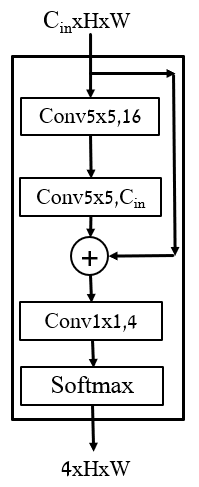
\includegraphics[height=60mm,width=3.5cm]{Figures/AttentionModUl.PNG}}
\caption{Attantion module structure used by SWASPP micro-architecture}
\label{attain}
\end{figure}
\end{center}
To fuse these feature maps produced by different pipeline of the SWASPP from the input feature map, an attention module is emerged. Attention module can be thought as a pixel level classification of which scale does this pixel it belongs to. Fig.~\ref{attain} illustrates the proposed attention module structure. Proposed attention module generates four heatmaps. The first three heatmaps correspond to the three scale feature maps while the remaining heatmap corresponds to the input feature map itself. These heatmaps are summed  up to one (\textit{i.e.,} for a  spatial position 
$(x, y)$, $\sum_{i =1}^{4} H(i,x,y) = 1$ where $H(i,x,y)$ is the $i$ heatmap produced by the attention module). To make sure this property holds, softmax function is used. 

The proposed mirco-architecture uses a pixel level weights produced by corresponding attention module rather than a single weight value for each scale. A single input CXR image may have multiple COVID-19 pneumonia scales which effectively lead to simply averaging the scale space when using single weight for each scale on scale space. In SWASPP, every convolution operation is followed by a BN and leakyReLU~\cite{krizhevsky2012imagenet} non-linearity except the re-projection layers that used to project back to the input space is not followed by nonlinearity. 
BN allows the use of larger learning rate~\cite{ioffe2015batch} and makes network stable during training~\cite{ioffe2015batch}. BN makes the loss landscape of the optimization problem significantly smoother~\cite{santurkar2018does}.
leakyReLU is used to reduce the vanishing gradient problem~\cite{krizhevsky2012imagenet}.
A bottleneck is introduced within both the attention module and multi-scale feature extractor pipeline. A bottleneck in SWASPP is used to project the input feature map of dimension $C_{in}\times H\times W$ to $32\times H\times W$ then re-project back to $C_{in}\times H\times W$. Multi-scale feature extraction is preformed on the projected dimension. Same logic is applied to the attention module where the input feature map is projected to a dimension of $16\times H\times W$.
This bottleneck allows the efficient use of model capacity and reduce the network computational complexity~\cite{huang2017densely}. It only allows the flow of important information and discarding irrelevant information. 

\subsection{Proposed CNN Architecture}
SWASPP is densely stacked~\cite{huang2017densely} together as Fig.~\ref{denseB} illustrates. This kind of connectivity allows implicit deep supervisions as each layer is effectively connected to the last layer using shorter path also facilitate feature reuse~\cite{huang2017densely} and gradient flow. Residual layers are easier to optimize if the required mapping is the identity mapping or simply near to it~\cite{he2016deep}. Densely stacked SWASPP is denoted by (DSWASPP). Convolutional part of proposed model consists of stacking six DSWASPP layers such that the first four layers are interconnected using maxpooling to reduce the spatial size and enlarge the Network receptive field. A single level Spatial Pyramid Pooling (SPP)~\cite{he2015spatial} is added after to produce a fixed size feature vector for a variable size input. SPP layer divides the input feature map into $10\times 10 = 100$ bins then performs a $max$ for each bin as an aggregation function. 
\begin{center}
\begin{figure}[htbp]
\centerline{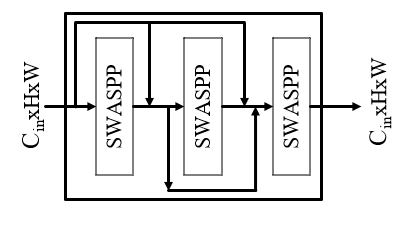
\includegraphics[height=30mm,width=6cm]{Figures/DensResd.PNG}}
\caption{Densely connected SWASPP (DSWASPP): is a stack of densely connected SWASPP, such that the output of any SWASPP is Concatenated to the input of all next layers. All the three layers produce an output of dimension of $C_{in} \times H \times W$.}
\label{denseB}
\end{figure}
\end{center}

The fixed length feature vector produced by SPP is used as an input to dropout~\cite{srivastava2014dropout} layer. Dropout layer randomly sets the activation of to $0$ with a probability of $0.5$. Dropout prevents the overfitting and reduce complex co-adaptation between the neurons allowing them to learn better representation~\cite{srivastava2014dropout}. It allow implicit ensempling of exponential number of sampled thin network from the original network which enhance the network performance~\cite{srivastava2014dropout}. The result of dropout layer is used as input to the classification network. Classification network consists of a fully connected layers with a $3$ Dense layers such that the output layer is 2-neuron for binary classification \textit{i.e)} COVID19 or not. Table~\ref{PCNN} shows the details of the proposed architecture.

\renewcommand{\arraystretch}{1.5}
\begin{table}[htbp]
    \caption{Proposed CNN architecture of methodology II}
    \begin{center}
    \begin{tabular}{|c|c|c|c|}
    \hline
    \textbf{Layer}&\multicolumn{3}{|c|}{\textbf{Proposed CNN Architecture of Methodology II}} \\
    \cline{2-4} 
    \textbf{Name} & \textbf{\textit{Input Shape}}& \textbf{\textit{Output Shape}}& \textbf{\textit{Param. Count}} \\
    \hline
    Input layer & - & $1 \times 320 \times 320$ & 0 \\
    \hline
    BatchNorm-1 & $1 \times 320 \times 320$ & $1 \times 320 \times 320$ & 2 \\
    \hline
    DSWASPP-1& $1 \times 320 \times 320$ & $32 \times 320 \times 320$ & 121,035  \\
    \hline
    Maxpooling-1& $32 \times 320 \times 320$ &$32 \times 160 \times 160$ & 0 \\
    \hline
    DSWASPP-2& $32 \times 160 \times 160$ & $64 \times 160 \times 160$ & 298,236  \\
    \hline
    Maxpooling-2 & $64 \times 160 \times 160$ & $64 \times 80 \times 80$ &0  \\
    \hline
    DSWASPP-3  & $64 \times 80 \times 80$ & $128 \times 80 \times 80$ & 604,956  \\
    \hline
    Maxpooling-3 & $128 \times 80 \times 80$ & $128 \times 40 \times 40$ & 0  \\
    \hline
    DSWASPP-4  & $128 \times 80 \times 80$ & $128 \times 80 \times 80$ & 784,092 \\
    \hline
    DSWASPP-5  & $128 \times 80 \times 80$ & $128 \times 80 \times 80$ & 784,092 \\
    \hline
    DSWASPP-6  & $128 \times 80 \times 80$ & $128 \times 80 \times 80$ & 784,092 \\
    \hline
    SPP-1 & $128 \times 80 \times 80$ & $12800$ & 0 \\
    \hline
    Dropout-1 & $12800$ & $12800$ & 0 \\
    \hline
    FC-1 & $12800$ & $128$ & 1,638,528 \\
    \hline
    FC-2 & $128$ & $128$ & 16,512 \\
    \hline
    FC-3 & $128$ & $64$ & 8,256 \\
    \hline
    FC-4 & $64$ & $2$ & 130 \\
    \hline
    Softmax & $2$ & $2$ & 0 \\
    \hline
    \hline
    \multicolumn{3}{|c|}{Total Number of Parameter}&5,040,571\\
    \hline
    \multicolumn{4}{c}{Any linear combination is followed by BN and leakyReLU nonlinearity}\\
    \multicolumn{4}{l}{excluding re-projection layer of the SWASPP modules}
    \end{tabular}
    \label{PCNN}
    \end{center}
    \end{table}

\section{Summary}

% CNN is a scale variant model. Many approaches were introduced to overcome this problem such as shared networks, feature pyramid network and atrous convolution. Atrous convolution increases the receptive field of the convolutional kernel without neither increasing the parameter number nor the computational complexity. Atrous convolution is used in the proposed work II to construct the scale space of the input feature. Attention mechanism is used to guide to process the most relevant part of the feature maps. To select the correct scale and fuse multiple scales of the input feature map a spatial attention module is used. A novel CNN architecture is proposed that internally produces multiscale feature maps which is further fused using attention based mechanism. Compact representation is learned via a bottleneck dimension which is introduced in both the multiscale feature extractor module and the attention module.

Convolutional Neural Networks (CNNs) have been widely used in computer vision tasks, including image classification, object detection, and segmentation. However, CNNs are known to be scale variant models, meaning that they can miss important features at different scales. To overcome this issue, various approaches have been proposed, such as shared networks, feature pyramid networks, and atrous convolution.
In this chapter, the proposed lightweight CNN architecture for COVID-19 detection is designed with the concept of spatial separability in mind. The spatial separability of the convolutional kernel is used to enforce the learning of linear kernels, which reduces the number of training parameters and improves computational efficiency. Essentially, the model is designed to recognize patterns in the data that are linearly separable, which enables the use of simpler and more efficient models.

The proposed architecture comprises separated kernel convolutional layers that are connected by a residual connection. The use of separated kernel convolutional layers helps to reduce the number of training parameters, while the residual connection improves network stability during the training process. The residual connection enables the model to retain important features while also discarding unimportant ones, which helps prevent overfitting.

Batch normalization is used in the proposed architecture to maintain network stability during the training process. The technique standardizes the inputs of each layer, which improves the convergence rate of the model. This is done by normalizing the layer inputs to have zero mean and unit variance, which helps prevent internal covariate shifts. Internal covariate shift refers to the change in the distribution of network activations that occurs during training, which can slow down the convergence rate.

In summary, the proposed lightweight CNN architecture for COVID-19 detection is based on the spatial separability of the convolutional kernel, with separated kernel convolutional layers connected by a residual connection. Batch normalization is used to maintain network stability during training, which improves the convergence rate of the model. By combining these techniques, the proposed architecture offers an efficient, accurate, and stable method for detecting COVID-19.

Atrous convolution, also known as dilated convolution, increases the receptive field of the convolutional kernel without increasing the number of parameters or computational complexity. In the proposed work II, atrous convolution is used to construct the scale space of the input feature, allowing the CNN to extract multiscale features.

Moreover, to select the correct scale and fuse multiple scales of the input feature map, a spatial attention module is used in the proposed work II. This attention mechanism guides the network to focus on the most relevant parts of the feature maps, which helps to improve the accuracy of the network.

To further enhance the performance of the network, a novel CNN architecture is proposed in which multiscale feature maps are internally produced and then fused using an attention-based mechanism. This approach leads to a compact representation of the input data via a bottleneck dimension introduced in both the multiscale feature extractor module and the attention module. Overall, these techniques and architectures help to improve the performance and accuracy of CNNs for computer vision tasks.
